

\tikzset{every picture/.style={line width=0.75pt}} %set default line width to 0.75pt        

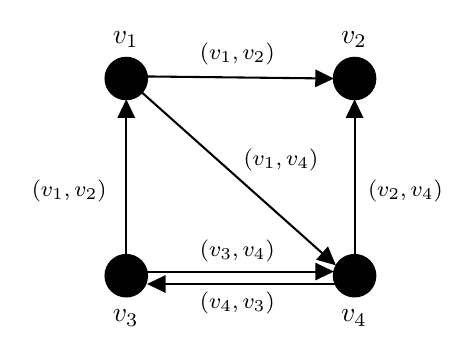
\begin{tikzpicture}[x=0.75pt,y=0.75pt,yscale=-1,xscale=1]
%uncomment if require: \path (0,186); %set diagram left start at 0, and has height of 186

%Straight Lines [id:da7523828398029215] 
\draw    (70,40) -- (157,40.97) ;
\draw [shift={(160,41)}, rotate = 180.64] [fill={rgb, 255:red, 0; green, 0; blue, 0 }  ][line width=0.08]  [draw opacity=0] (8.93,-4.29) -- (0,0) -- (8.93,4.29) -- cycle    ;
%Straight Lines [id:da6810560947997366] 
\draw    (60,134) -- (60,54) ;
\draw [shift={(60,51)}, rotate = 450] [fill={rgb, 255:red, 0; green, 0; blue, 0 }  ][line width=0.08]  [draw opacity=0] (8.93,-4.29) -- (0,0) -- (8.93,4.29) -- cycle    ;
%Straight Lines [id:da13593621053018157] 
\draw    (60,41) -- (158.76,129) ;
\draw [shift={(161,131)}, rotate = 221.7] [fill={rgb, 255:red, 0; green, 0; blue, 0 }  ][line width=0.08]  [draw opacity=0] (8.93,-4.29) -- (0,0) -- (8.93,4.29) -- cycle    ;
%Straight Lines [id:da7020714410789375] 
\draw    (170,130) -- (170,54) ;
\draw [shift={(170,51)}, rotate = 450] [fill={rgb, 255:red, 0; green, 0; blue, 0 }  ][line width=0.08]  [draw opacity=0] (8.93,-4.29) -- (0,0) -- (8.93,4.29) -- cycle    ;
%Shape: Circle [id:dp03304258230702484] 
\draw  [color={rgb, 255:red, 0; green, 0; blue, 0 }  ,draw opacity=1 ][fill={rgb, 255:red, 0; green, 0; blue, 0 }  ,fill opacity=1 ] (160,136) .. controls (160,130.48) and (164.48,126) .. (170,126) .. controls (175.52,126) and (180,130.48) .. (180,136) .. controls (180,141.52) and (175.52,146) .. (170,146) .. controls (164.48,146) and (160,141.52) .. (160,136) -- cycle ;
%Shape: Circle [id:dp7633189619087324] 
\draw  [color={rgb, 255:red, 0; green, 0; blue, 0 }  ,draw opacity=1 ][fill={rgb, 255:red, 0; green, 0; blue, 0 }  ,fill opacity=1 ] (50,136) .. controls (50,130.48) and (54.48,126) .. (60,126) .. controls (65.52,126) and (70,130.48) .. (70,136) .. controls (70,141.52) and (65.52,146) .. (60,146) .. controls (54.48,146) and (50,141.52) .. (50,136) -- cycle ;
%Shape: Circle [id:dp47599843876160874] 
\draw  [color={rgb, 255:red, 0; green, 0; blue, 0 }  ,draw opacity=1 ][fill={rgb, 255:red, 0; green, 0; blue, 0 }  ,fill opacity=1 ] (160,41) .. controls (160,35.48) and (164.48,31) .. (170,31) .. controls (175.52,31) and (180,35.48) .. (180,41) .. controls (180,46.52) and (175.52,51) .. (170,51) .. controls (164.48,51) and (160,46.52) .. (160,41) -- cycle ;
%Shape: Circle [id:dp8036256762510467] 
\draw  [color={rgb, 255:red, 0; green, 0; blue, 0 }  ,draw opacity=1 ][fill={rgb, 255:red, 0; green, 0; blue, 0 }  ,fill opacity=1 ] (50,41) .. controls (50,35.48) and (54.48,31) .. (60,31) .. controls (65.52,31) and (70,35.48) .. (70,41) .. controls (70,46.52) and (65.52,51) .. (60,51) .. controls (54.48,51) and (50,46.52) .. (50,41) -- cycle ;
%Straight Lines [id:da523220310179759] 
\draw    (60,134) -- (157,134) ;
\draw [shift={(160,134)}, rotate = 180] [fill={rgb, 255:red, 0; green, 0; blue, 0 }  ][line width=0.08]  [draw opacity=0] (8.93,-4.29) -- (0,0) -- (8.93,4.29) -- cycle    ;
%Straight Lines [id:da5511445342877679] 
\draw    (170,140) -- (73,140) ;
\draw [shift={(70,140)}, rotate = 360] [fill={rgb, 255:red, 0; green, 0; blue, 0 }  ][line width=0.08]  [draw opacity=0] (8.93,-4.29) -- (0,0) -- (8.93,4.29) -- cycle    ;

% Text Node
\draw (52,17) node [anchor=north west][inner sep=0.75pt]    {$v_{1}$};
% Text Node
\draw (162,17) node [anchor=north west][inner sep=0.75pt]    {$v_{2}$};
% Text Node
\draw (52,151) node [anchor=north west][inner sep=0.75pt]    {$v_{3}$};
% Text Node
\draw (162,151) node [anchor=north west][inner sep=0.75pt]    {$v_{4}$};
% Text Node
\draw (94,22.4) node [anchor=north west][inner sep=0.75pt]  [font=\footnotesize]  {$( v_{1} ,v_{2})$};
% Text Node
\draw (115,73.4) node [anchor=north west][inner sep=0.75pt]  [font=\footnotesize]  {$( v_{1} ,v_{4})$};
% Text Node
\draw (175,88.4) node [anchor=north west][inner sep=0.75pt]  [font=\footnotesize]  {$( v_{2} ,v_{4})$};
% Text Node
\draw (13,88.4) node [anchor=north west][inner sep=0.75pt]  [font=\footnotesize]  {$( v_{1} ,v_{2})$};
% Text Node
\draw (94,117.4) node [anchor=north west][inner sep=0.75pt]  [font=\footnotesize]  {$( v_{3} ,v_{4})$};
% Text Node
\draw (94,142.4) node [anchor=north west][inner sep=0.75pt]  [font=\footnotesize]  {$( v_{4} ,v_{3})$};


\end{tikzpicture}